% Source-faithful schematic draft: 2006 Chongqing Science Q9, PDF p.1 (printed p.284).
% Source ID: src-5abd831561d7d4fa968c5bf0deb634e0d666376fd8cc90967cf30d301e77a351
% Source SHA-256: 211d79b8676187c7e4a98c71d7eae5eadd28b2e5aaf9237fefd55a791241faa3
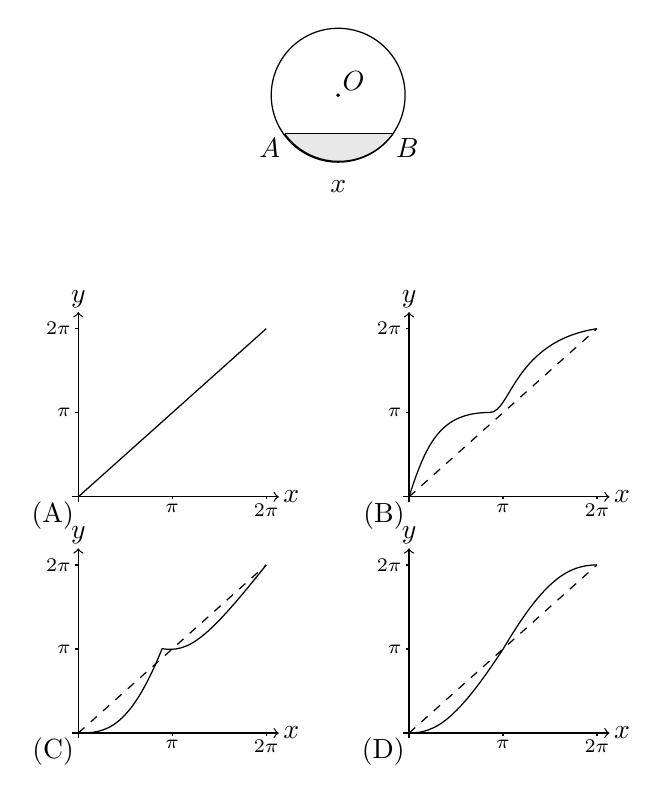
\begin{tikzpicture}[line width=0.45pt,every node/.style={inner sep=1.4pt}]
% Source circle, chord AB, shaded circular segment, center O and arc-length label x.
\begin{scope}[xshift=3.3cm,yshift=5.1cm]
 \draw (0,0) circle (0.85);
 \coordinate (A) at (-0.68,-0.49); \coordinate (B) at (0.68,-0.49);
 \fill[gray!18] (A) arc[start angle=216,end angle=324,radius=0.85] -- (B) -- cycle;
 \draw (A) arc[start angle=216,end angle=324,radius=0.85]; \draw (A)--(B);
 \fill (0,0) circle (0.025) node[above right] {$O$};
 \node[below left] at (A) {$A$}; \node[below right] at (B) {$B$}; \node[below] at (0,-1.03) {$x$};
\end{scope}
% Four graph options in a 2 by 2 layout. The dashed y=x reference is visible in B,C,D.
% Each coordinate system represents x,y from 0 to 2pi; curves are qualitative sketches.
\begin{scope}[xshift=0cm,yshift=0cm,x=0.38cm,y=0.34cm]
 \draw[->] (-0.2,0)--(6.7,0) node[right] {$x$}; \draw[->] (0,-0.2)--(0,6.9) node[above] {$y$};
 \draw (0,0)--(6.28,6.28); \node[below left] at (0,0) {(A)};
 \foreach \t/\lab in {3.14/\pi,6.28/2\pi} {\draw (\t,0)--(\t,-0.1) node[below] {\scriptsize $\lab$}; \draw (0,\t)--(-0.1,\t) node[left] {\scriptsize $\lab$};}
\end{scope}
\begin{scope}[xshift=4.2cm,yshift=0cm,x=0.38cm,y=0.34cm]
 \draw[->] (-0.2,0)--(6.7,0) node[right] {$x$}; \draw[->] (0,-0.2)--(0,6.9) node[above] {$y$};
 \draw[dashed] (0,0)--(6.28,6.28); \draw (0,0) .. controls (0.6,2.1) and (1.1,3.15) .. (2.7,3.15) .. controls (3.4,3.15) and (3.5,5.8) .. (6.28,6.28); \node[below left] at (0,0) {(B)};
 \foreach \t/\lab in {3.14/\pi,6.28/2\pi} {\draw (\t,0)--(\t,-0.1) node[below] {\scriptsize $\lab$}; \draw (0,\t)--(-0.1,\t) node[left] {\scriptsize $\lab$};}
\end{scope}
\begin{scope}[xshift=0cm,yshift=-3.0cm,x=0.38cm,y=0.34cm]
 \draw[->] (-0.2,0)--(6.7,0) node[right] {$x$}; \draw[->] (0,-0.2)--(0,6.9) node[above] {$y$};
 \draw[dashed] (0,0)--(6.28,6.28); \draw (0,0) .. controls (0.9,0) and (1.7,0.1) .. (2.8,3.15) .. controls (3.7,3.0) and (4.3,3.5) .. (6.28,6.28); \node[below left] at (0,0) {(C)};
 \foreach \t/\lab in {3.14/\pi,6.28/2\pi} {\draw (\t,0)--(\t,-0.1) node[below] {\scriptsize $\lab$}; \draw (0,\t)--(-0.1,\t) node[left] {\scriptsize $\lab$};}
\end{scope}
\begin{scope}[xshift=4.2cm,yshift=-3.0cm,x=0.38cm,y=0.34cm]
 \draw[->] (-0.2,0)--(6.7,0) node[right] {$x$}; \draw[->] (0,-0.2)--(0,6.9) node[above] {$y$};
 \draw[dashed] (0,0)--(6.28,6.28); \draw (0,0) .. controls (0.9,0) and (1.6,0.5) .. (3.15,3.15) .. controls (4.4,5.5) and (5.2,6.28) .. (6.28,6.28); \node[below left] at (0,0) {(D)};
 \foreach \t/\lab in {3.14/\pi,6.28/2\pi} {\draw (\t,0)--(\t,-0.1) node[below] {\scriptsize $\lab$}; \draw (0,\t)--(-0.1,\t) node[left] {\scriptsize $\lab$};}
\end{scope}
\end{tikzpicture}
